% "pdf"

\documentclass[a4paper,12pt]{article}

\usepackage[french]{babel}
\usepackage[T1]{fontenc}
\usepackage[utf8x]{inputenc}

\usepackage[margin=2cm]{geometry}
\usepackage{pifont}

\usepackage[colorlinks=true,
            linkcolor=black]{hyperref}
\usepackage{titletoc}
\usepackage{titlesec}

\usepackage{soul}
% \usepackage{ulem}

\usepackage[french, lined,ruled]{algorithm2e}

\title{\Huge\textbf{Rapport de Phase 1 du Groupe 1}}
\author{Lemarchand Benoît \& Megna Anaël \& Shimi Adam}
\date{Jeudi, 7 Mai 2015}

\usepackage{fancyhdr}
\pagestyle{fancy}
\renewcommand{\headrulewidth}{0pt}
\lfoot{} \cfoot{} \rfoot{\thepage} \lhead{} \chead{} \rhead{}

\usepackage{amsmath}
\usepackage{amssymb}
\usepackage{amsthm}
\usepackage{mathtools}
\usepackage{mathrsfs}
\usepackage{stmaryrd}
\usepackage{esint}
\usepackage{esvect}
\usepackage{multirow}

\DeclareMathOperator{\Tr}{Tr}

\newtheorem*{remark}{Remarque}

\usepackage{listings}

\newcommand{\norme}[1]{\left\Vert #1\right\Vert}

\renewcommand{\phi}{\varphi}
\renewcommand{\epsilon}{\varepsilon}

\setlength{\parindent}{1em}

\begin{document}

\begin{titlepage}
  \maketitle
  \thispagestyle{empty}
  \tableofcontents
\end{titlepage}

\section{Reconstruction et Classification de la solution d'un modèle
atmosphérique simplifié}

\subsection{Détermination de $\alpha$}

Résoudre le problème de minimisation en $\alpha$
$\displaystyle \min_{\alpha \in \mathbb{R}^{n_d}} \|U_{|t=0}.\alpha - Z_0\|_2$
revient à trouver $\alpha \in \mathbb{R}^{n_d}$ tel que
$\displaystyle U_{|t=0}^T.U_{|t=0}.\alpha = U_{|t=0}^T.Z_0$ (équations
normales).

Or $U_{|t=0}^T.U_{|t=0}$ est, de manière évidente, une matrice symétrique
positive et, de plus, par construction de $U$, ses valeurs propres sont non
nulles d'où son caractère défini. L'algorithme de la \og steepest descent \fg
nous semble donc adaptée pour deux points.

\begin{itemize}
    \item Nous pouvons adapter le résidu de la solution. En effet, la méthode
        de la puissance itérée permet de choisir la précision de l'espace
        vectoriel d'approximation. Ainsi nous pouvons choisir une précision
        cohérente.
    \item Chaque tour de boucle à une complexité en temps de l'ordre de
        $\mathcal{O}(n_d^2)$. Chaque étape est très rapide dès que
        l'approximation est suffisamment efficace.
\end{itemize}


\begin{algorithm}[H]
    $\epsilon = value$\;
    $\alpha = vector$\;
    $U'_0 = U_0^T . U_0$\;
    $Z'_0 = U_0^T . Z_0$\;
    $r = Z'_{0} - U'_0 . \alpha$\;
    \While{ $\displaystyle \frac{\|r\|_2}{\|Z'_0\|_2}  > \epsilon$ }{
        $\displaystyle \lambda = \frac{r^T.r}{(U_0 . r)^T . (U_0 . r)}$\;
        $\alpha = \alpha + \lambda r$\;
        $r = Z'_0 - U'_0 . \alpha$\;
    }
    \caption{Détermination de $\alpha$}
\end{algorithm}

\subsection{Classification d'une solution}

Classifier une observation revient à minimiser la distance qui la sépare de sa
projection dans un panel de solutions généré avec une classe particulière, c'est
à dire, trouver $GW$ qui offre un panel de solutions proche de l'observation.

\begin{algorithm}
    \DontPrintSemicolon
    \For{$i \in \mathbb{N}_3$}{
        Calculer $U_i$\;
        $Z_{obs,i} = F_{obs} - \bar{F}_i$\;
        $\pi_i = \|Z_{obs,i} - U_i^T.U_i.Z_{obs,i}\|_2$\;
    }
    \caption{Algorithme de classification}
\end{algorithm}

Connaître la classe de l'observation revient alors simplement à prendre $i$ tel
que $\pi_i$ soit le plus petit des trois.

\newpage
\section{Influence des paramètres sur les solutions}

\subsection{Sur la classification}

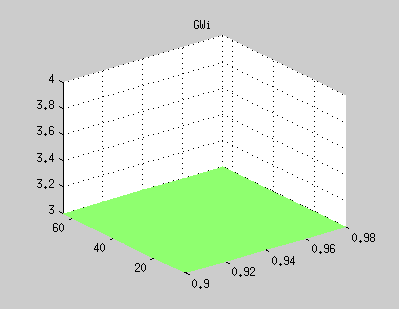
\includegraphics[width=10em, height=10em]{class.png}
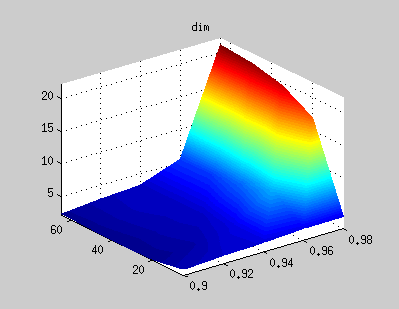
\includegraphics[width=10em, height=10em]{dimension.png}
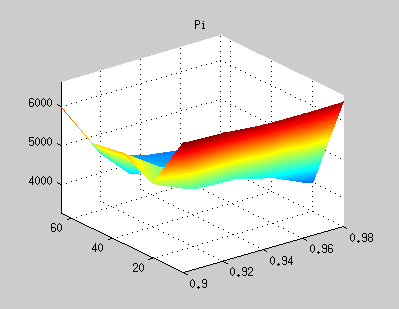
\includegraphics[width=10em, height=10em]{distance.png}

Voici trois graphes représentant respectivement l'évolution de $GWi$ la classe de
l'observation, de la dimension du sous espace, et de la distance entre le
projeté et le sous espace, ceci en fonction de $percentInfo$ et de $N_{ens}$.

\paragraph{}
On voit donc que les modification de ces paramètres n'influencent pas sur
l'obtention de la classe de l'observation.

Le graphique n'étant pas affiché, il faut néanmoins savoir que le temps
d'exécution croît grandement avec $N_{ens}$, résultat que l'on pouvait deviner.
Il peut être alors acceptable de travailler avec un $percentInfo$ et un
$N_{ens}$ bas car le résultat qui nous intéresse dans cette partie ne varie pas.
(Ce qui ne peut pas être accepté lors de la reconstruction car l'erreur entre le
modèle et la solution reconstruite grandirait).

\paragraph{}
On voit aussi qu'une augmentation de $percentInfo$ implique une augmentation de
la dimension du sous espace sur lequel on projettera la solution, alors que
$N_{ens}$ ne semble pas avoir d'effet sur ce résultat.

\paragraph{}
Pour finir, on remarquera que la distance entre l'observation et le sous espace
diminue lorsque $percentInfo$ et $N_{ens}$ augmentent.

\subsection{Suite des influences}

Pour des raisons de temps, les graphes ne sont générés que sur 5 valeurs de
$percentInfo$ et de $N_{ens}$, avec uniquement 5 générations aléatoires pour
chacun d'entre elles.
Idéalement, nous aurions voulu étendre la plage de test à 15 valeurs de
$percentInfo$ et de $N_{ens}$, avec pour chacune d'elles, une vingtaine de
générations aléatoires afin d'obtenir un résultat plus représentatif.
Seulement, ces test étant très longs, le script permettant de les répartir sur
les machines de l'n7 n'a été terminé qu'à l'instant (jeudi 7, 23h30), sa
réalisation étant plus complexe que ce que nous imaginions.

\paragraph{}
Nous n'avons donc pas eu le temps d'adapter ces test pour la reconstruction.

Il est cependant évident que plus $percentInfo$ et $N_{ens}$ sont élevés, plus
l'erreur relative sera faible.

\newpage
\section{Méthode dérivée de la puissance itérée, analyse et implémentation}

    \subsection{Avantages et inconvénients de la méthode}

        \begin{remark}[Complexité en temps du calcul matriciel]
        Ici, nous utilisons les routines de calcul matriciel de MATLAB, qui
        viennent de BLAS.\footnote{Voir la routine DGEMM,
        \url{http://en.wikipedia.org/wiki/Basic_Linear_Algebra_Subprograms}}
        Étant donné que ces routines, quoique optimisées pour s'adapter au
        matériel et réduire les temps de calcul, n'implémentent ni l'algorithme
        de Strassen en $\mathcal{O}(n^{2.807})$ ni aucun des développements
        récents dans le domaine qui vont jusqu'au $\mathcal{O}(n^{2.3728642})$ de
        Virginia V. Williams et au $\mathcal{0}(n^{2.3728639})$ de LeGall, nous
        supposerons que la complexité en temps d'une multiplication matricielle
        de MATLAB est en $\mathcal{O}(n^3)$ pour une matrice de
        $\mathbb{R}^{n*n}$ et $\mathcal{O}(nmk)$ pour des matrices de
        $\mathbb{R}^{n*m}$ et $\mathbb{R}^{m*k}$.
        \end{remark}

        Ici, nous analysons l'algorithme de la puissance itérée adapté aux
        sous-espaces propres, à la fois en terme d'avantages et d'inconvénients.
        Évidemment, ces termes n'ont de sens qu'au niveau d'une comparaison.

        D'où le choix d'un algorithme dit \og de base \fg, à l'aune duquel nous
        pourrons analyser celui qui fait l'objet de cette section.  Les
        particularités de cet algorithme \og de base \fg sont :

        \begin{itemize}
        \item Il calcule toutes les valeurs singulières et tous les vecteurs
            singuliers.

        \item Il est basé, d'après la documentation de
            MATLAB\footnote{MATLAB utilise la routine $svd$ de LIPACK, dont
            l'algorithme est expliqué dans J. Demmel, W. Kahan
            \emph{Accurate Singular Values of Bidiagonal Matrices},
            submitted to SIAM J.Sci.Stat.Comput., v.11, n.5, pp.873-912,
            1990}, sur l'application successive de transformation de Householder
            et de Rotation de Givens, avant d'appliquer une methode itérative de
            calcul des valeurs et vecteurs singuliers pour une matrice
            bidiagonale.

        \item Sa complexité asymptotique en temps est, toujours d'après
            l'implémentation MATLAB, en $\mathcal{O}(MaxIter*(n*m^2))$, où
            $MaxIter$ est le nombre d'itérations maximal de la seconde
            partie de l'algorithme.

        \item Celle en espace, basée sur celles des différentes étapes de
            l'algorithme, est en $\mathcal{O}(n*m)$.
        \end{itemize}

    \bigskip

        Par comparaison, notre nouvel algorithme a pour caractéristiques :

        \begin{itemize}
        \item Il calcule uniquement les valeurs singulières et les vecteurs
            singuliers à gauche nécessaire d'après le pourcentage d'information
            demandé.

        \item En ce qui concerne la complexité en temps pour A $\in
            \mathbb{R}^{m*m}$, nous obtenons comme formule asymptotique
            $\mathcal{O}(MaxIter*(n*m^2))$. En effet, toutes les matrices
            impliquées dans notre algorithme sont de taille $n*m$, excepté $A$.
            Nous en déduisons d'après la remarque sur la complexité que
            l'ensemble des calculs matriciels de notre algorithme est en
            $\mathcal{O}(n*m^2)$.  Ajoutons a cela la partie itérative, bornée
            par $MaxIter$, et nous obtenons cette complexité.

        \item Quand à la complexité en espace, la version naïve de l'algorithme,
            qui consiste à calculer $A$ avant toute chose, nous donne une
            complexité en $\mathcal{O}(m^2)$, étant donné que c'est la matrice
            la plus volumineuse.
        \end{itemize}

    \bigskip

        Le premier point de comparaison est celui du temps de calcul. Comme nous
        l'avons vu, asymptotiquement, les deux algorithmes se comportent
        similairement en terme de temps. Cependant, notre algorithme ne va pas
        calculer toutes les valeurs singulières, sauf dans de très rares cas. Il
        semble donc sensé de supposer que si les deux algorithmes se valent dans
        le pire des cas, le notre a un léger avantage sur $svd$ lorsque
        $PercentTrace$ est relativement éloigné de 1.

        Ensuite vient la question de l'espace. Ici, clairement, notre algorithme
        a un désavantage lié au calcul explicite et au stockage de $A$, qui fait
        augmenter la complexité asymptotique en espace. Si l'on considère en
        plus que $m$ dans le cas pratique que nous implémentons ici est de
        l'ordre de $10^5$, ce désavantage est écrasant. Nous verrons dans la
        sous-section suivante comment se passer du stockage de $A$.

        Enfin, en ce qui concerne les avantages moins significatifs de notre
        algorithme, il y a le fait que dans la majorité des cas, il stocke moins
        de valeurs singulières que $svd$. Et dans tous les cas, il stocke moins
        de vecteurs singuliers, étant donné qu'il ne calcule à aucun moment les
        vecteurs singuliers à droite. Nous pouvons aussi remarquer que notre
        algorithme sort directement un sous-espace "singulier", tandis qu'il
        faut reconstruire celui-ci avec la sortie de $svd$.

    \subsection{Implémentation de l'algorithme}

        Comme expliqué dans la sous-section précédente, l'utilisation naïve de
        l'algorithme dérivé de la puissance itérée pour remplacer $svd$
        nécessite le calcul de $A = Z*Z^T$, dont l'ordre de grandeur du nombre
        de coefficients est de $10^{10}$. Ceci fait que le calcul même de $A$
        entraine un overflow dans MATLAB, nous forçant à adapter l'algorithme
        pour l'utiliser.

        Voici les moments où nous avons dû modifier l'algorithme fourni pour
        éviter de calculer $A$ :

        \begin{itemize}
        \item Le calcul de $Y = A^p*V$. Ici, il suffit de remplacer $A$ par
            $Z*Z^T$, et d'effectuer les calculs. A aucun moment les matrices
            intermédiaires n'auront une taille supérieure à $n*m$, ce qui est
            assez petit pour ne pas causer d'overflow dans MATLAB.

        \item Le calcul du coefficient de Rayleigh $H = V^T*A*V$. Ici, pour
            gagner en espace, il suffit de décomposer $H = V^T*Z*Z^T*V =
            (Z^T*V)^T*(Z^T*V)$. Nous en déduisons que calculer $Z^T*V$ puis
            d'une transposition et d'un produit matriciel pour calculer le
            coefficient de Rayleigh.

        \item Le critère d'arrêt pour le calcul d'une valeur propre,
            $\displaystyle \frac{\norme{A*v_i - \lambda_i*v_i}}{\norme{A}}$.
            Le fait que $A$ soit une matrice symétrique nous permet de savoir,
            d'après le théorème spectral, que $\norme{A} = \lambda_1$, où
            $\lambda_1$ est la plus grande valeur propre de $A$. Pour ce qui est
            du dividende, il nous suffit de faire 2 produits matriciels (par
            $Z^T$ et $Z$) à la place d'un seul, puis de calculer la norme.

            Cependant, étant donné qu'il nous faut $\norme{A}$ dès la première
            itération de l'algorithme, avant donc d'avoir calculé la plus grande
            valeur singulière, nous appliquons la propriété bien connue que
            $Z*Z^T$ et $Z^T*Z$ ont toutes deux les mêmes valeurs propres, et
            sont toutes deux diagonalisables. Nous en déduisons que $\norme{A} =
            \norme{Z^T*Z}$, avec $Z^T*Z \in \mathbb{R}^{n*n}$, donc calculable
            sans overflow.

        \item Le critère d'arrêt pour l'algorithme en lui même doit être
            modifié. L'intuition derrière cette nécessitée est le fait que
            lorsque la plus grande valeur propre est sensiblement plus
            grande que les autres,
            $\displaystyle \frac{\sum\limits_{i=1}^n \lambda_i}{\Tr(A)}$
            tend à être plus grand que le résultat de l'équation (1), causant
            l'arrêt prématuré de l'algorithme.

            Nous pouvons prendre comme exemple le cas où n = 4, les valeurs
            propres calculées pour le moment valent 4 et 1 (d'où ici k = 2),
            $\Tr(A) = 7$ et $\lambda_{k+1} = 1$. Ainsi, le critère d'arrêt non
            modifié donne 5/7, tandis que l'équation 1 donne 1/2. Il suffit donc
            que $PercentInfo$ se trouve dans l'intervalle $[1/2,5/7]$ pour que
            l'algorithme soit faussé.

            Nous en concluons que pour avoir une implémentation fonctionnelle de
            l'algorithme, il nous faut utiliser le critère d'arrêt suivant :
            $\displaystyle \frac{\sigma_{k+1}}{\sigma_1} \leq
            1 - PercentInfo$ comme exprimé dans l'Equation (1). Le défaut de
            ce critère étant qu'il nécessite de calculer une valeur propre de
            plus avant d'arrêter. Mais il a l'avantage d'être correct et
            d'être utilisable sans overflow ni temps de calcul trop important.
        \end{itemize}
    \bigskip

        Il nous reste maintenant à écrire le pseudo-code de l'algorithme adapté.

        \begin{algorithm}[H]
            \DontPrintSemicolon
            $V = matrice\ orthogonale\ quelconque \in \mathbb{R}^{m*n}$\;
            $niter = 0$\;
            $converged = 0$\;
            $PercentReached = 0$\;
            $normeA = \norme{Z^T*Z}$\;
            \Repeat{$PercentReached \leq PercentInfo$ or $niter < MaxIter$}{
                \For{$i=1, p$}{
                    $V = Z^T*Y$\;
                    $V = Z*Y$\;
                }
                $V = \mathrm{Gram-Schmidt}(V)\footnote{Nous ne rappellons pas l'algorithme d'orthogonalisation de Gram-Schmidt, mais celui-çi est implémenté dans le code}$\;
                $H = Z^T*V$\;
                $H = H^T*H$\;
                $[X,\Lambda] = decomposition\ spectrale\ de\ H$\;
                $[X,\Lambda] = ordonnancement\ decroissant\ de\ [X,\Lambda]$\;
                $V = V*X$\;
                \For {$i=converged + 1, n$}{
                    \eIf{$\displaystyle \frac{\norme{Z*Z^T*V(i) - \Lambda(i,i).V(i)}}{normeA} \leq \epsilon$}{
                        $converged = converged + 1$\;
                        $\displaystyle PercentReached = 1 - \frac{\norme{Z - \sum\limits_{j=1}^i \sqrt[4]{\Lambda(i,i)}V(i)V(i)^TZ^T}}{\sqrt{normeA}}$\;
                    } {
                        break\;
                    }
                }
                $niter = niter + 1$\;
            }
            \caption{Méthode du sous-espace singulier dominant}
        \end{algorithm}

        \subsection{Commentaires}

        Il ne reste plus grand chose à dire sur cet algorithme, si ce n'est
        qu'il est moins rapide que $svd$, tout en étant aussi efficace. Nous
        supposons que cela vient du fait que $svd$ est optimisée par des appels
        à des langages plus rapides que MATLAB, à l'image du FORTRAN ou du C.
        Il nous semble donc que ce n'est qu'une question de temps avant que
        notre méthode soit aussi rapide que $svd$.


\end{document}
